\section{The ElGamal cryptosystem}
The ElGamal cryptosystem was proposed by Taher ElGamal in 1985 as an extension to the Diffie-Hellman protocol which can be applied in other cyclic groups, such as \textbf{Galois fields}. 

It is a public-key encryption algorithm, based on the intractability of the discrete logarithm, and considered over the group $\mathbb{Z}^*_p$ with $p$ prime.

Its key aspect is the \textbf{randomized encryption}, adding a layer of security, and its principal applications are establishing a secure channel for key sharing and message encryption. 

The ElGamal algorithm was proposed to remedy one flaw of the Diffie-Hellman key exchange: it requires interaction of both parties to calculate a common private key. This can constitute in a problem in case they are not able to interact, due to delays in transmission or unavailability of receiver.

The random exponent is therefore introduced to replace the private exponent of the receiving entity, so that it does not have to take part in the exchange.

\subsection{From Diffie-Hellman to ElGamal}
ElGamal follows immediately from Diffie-Hellman: to send an encrypted message $x$, Alice must perform a key exchange to derive a shared key $k_M$. However, as previously stated, only the receiver needs to create a key in advance and publish it.

A large prime $p$ and a primitive element $\alpha$ need to be generated, to whom ElGamal adds a random multiplicative mask to encrypt:
$$y \equiv x \cdot k_M \mod p$$

\begin{figure}[h]
	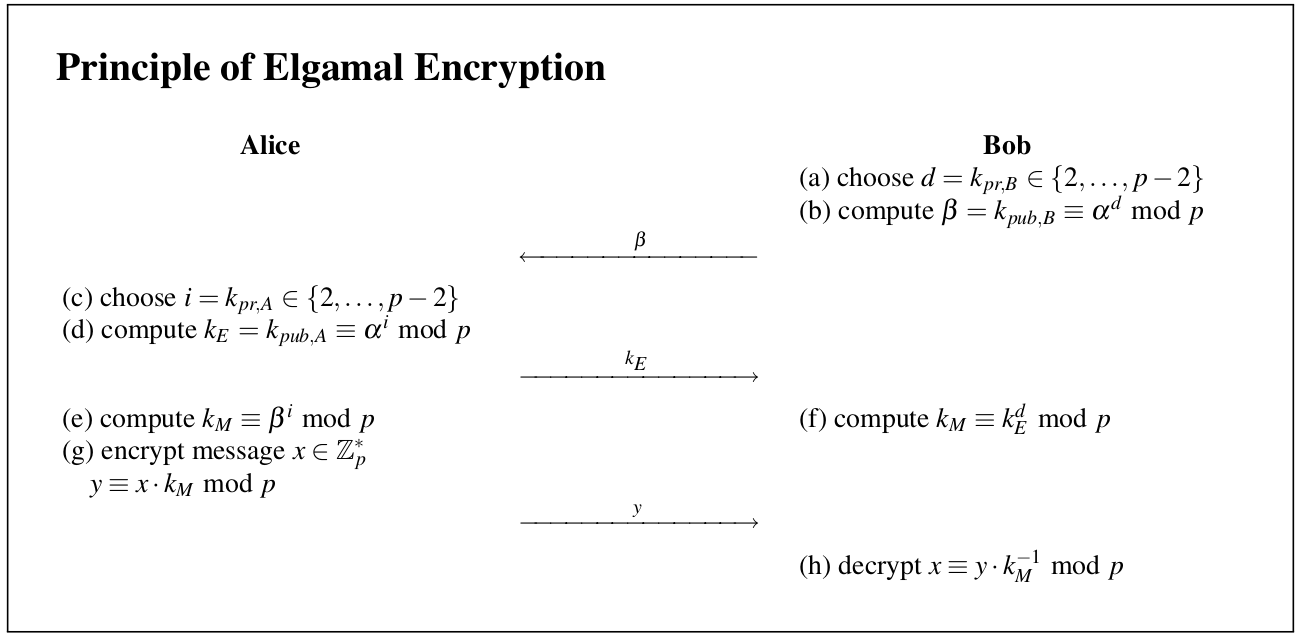
\includegraphics[scale=0.35]{ElGamalPrinciplePaar.png}
	\centering
\end{figure}

This protocol is similar to Diffie-Hellman: the private and public keys of Bob are computed the same way, and do not change over time, however Alice has to generate a new pair for the encryption of every message.

The key $k_E$ is \textbf{ephemeral}, meaning that it only exists temporarily, and $k_M$ is the joint key for masking the plain text. To encrypt a message, Alice multiplies the plaintext message $x$ by $k_M$ and Bob reverses this operation using the inverse mask.

\subsection{Protocol}
ElGamal encryption method works thanks to an important property of cyclic groups: given $k_M \in \mathbb{Z}^*_p$, every message $x$ maps to another cipher text computing $k_M \cdot x$, and random values allow to obtain the \textit{same probability} for every cipher text. 

\begin{figure}[h]
	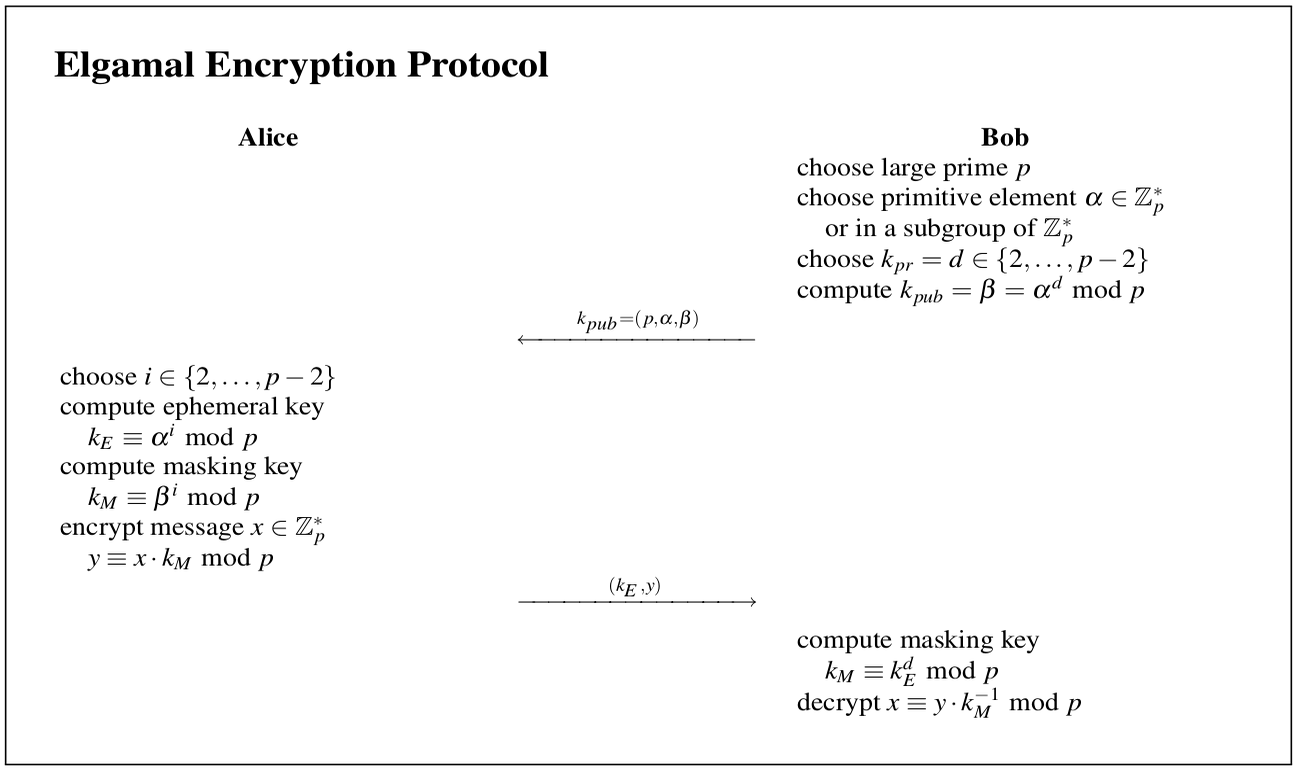
\includegraphics[scale=0.35]{ElGamalProtocolPaar.png}
	\centering
\end{figure}

The actual protocol is composed by three phases: \textbf{setup}, \textbf{encryption} and \textbf{decryption}. It starts by fixing a very large finite field $\mathbb{Z}^*_p$ and an element $\alpha \in \mathbb{Z}^*_p$ (preferably, but not necessarily a generator). 

Supposing an use of plain text message units with numerical equivalents in $\mathbb{Z}^*_p$, each user $A$ randomly chooses an integer $i$ in the range $0 < i < p - 1$. This integer $i$ is the secret deciphering key, while the public enciphering key is the element $k_E = \alpha^i \in \mathbb{Z}^*_p$.	

To send a message $y$ to the user $A$, an integer $d$ is chosen at random, and $A$ is sent the pair of elements:
$$(\alpha^d, y\alpha^{id})$$
$\alpha^{id} = k_E^d$ can be computing without knowing $i$ simply by raising $\alpha$ by the $d$-th power. Now Alice, who is aware of $i$, can recover $y$ from this pair simply by raising the first element $\alpha^d$ to the $i$-th power and dividing the result by the second element.

Public keys can be obtained in any way, for instance from key servers or unencrypted means. There is no security issues involved in this transmission, as the only secret is the exponent and therefore computationally infeasible.

In other words, the message is being masked but also contains a way to be recovered only by someone knowing the initial value $i$. 

The Diffie-Hellman sequence of operations is rearranged, since Bob receives only one message from Alice containing the ephemeral key and the encrypted text. In this case, however, the couple $(k_E, y)$ is generally \textbf{twice as long} as the message, since parameters have a bit length of $\lceil\log_2p\rceil$.

\subsubsection{Example}
Alice wants to send the message $x = 26$.

Bob generates $p = 29$ and $\alpha = 2$, then chooses $k_{pr, B} = d = 12$ to compute $\beta = \alpha^d \equiv 7 \mod 29$.

Alice receives the triple $k_{pub, B} = (p, \alpha, \beta) = (29, 2, 7)$, chooses $i = 5$ and then uses those to obtain the two temporary keys:
\begin{enumerate}
	\item $k_E = \alpha^i \equiv 3 \mod 29$
	\item $k_M = \beta^i \equiv 16 \mod 29$
\end{enumerate}
Alice encrypts $y = x \cdot k_M \equiv 10 \mod 29$, and sends it to Bob with the ephemeral key $k_E$.

Bob computes $k_M = k_E^d \equiv 16 \mod 29$, which is the same as Alice, and uses it to decrypt the message:
$$x = y \cdot k^{-1}_M \equiv 10 \cdot 20 \equiv 26 \mod 29$$

\subsection{Proof}
Assuming the value $d_{k_{pr}}(k_E, y)$ actually returns the original message $x$:
\begin{equation}
\begin{split}
d_{k_{pr}}(k_E, y) &\equiv y \cdot (k_M)^{-1} \mod p \\
&\equiv [x \cdot k_M] \cdot (k_E^d)^{-1} \mod p \\
&\equiv [x \cdot (\alpha^d)^i]^{-1} \mod p \\
&\equiv x \cdot \alpha^{d \cdot i - d \cdot i} \mod p \\
&\equiv x \mod p
\end{split}
\end{equation}

\subsection{Practical applications}
ElGamal encryption is not widely used in practice, since one of the best known practices to break it exploits its malleability: the ciphertext $(k_E, y)$ can be replaced with $(k_e, sy)$ for some integer $s$.

The receiver therefore then computes:
\begin{equation}
\begin{split}
d_{k_{pr}}(k_E, sy) &\equiv sy \cdot (k_M)^{-1} \mod p \\
&\equiv s \cdot (x \cdot k_M) \cdot k_M^{-1} \mod p \\
&\equiv sx \mod p
\end{split}
\end{equation}

The decrypted text is also a multiple of $s$, and although an attacker would not be able to decrypt the message, he is able to manipulate it for instance doubling or tripling the value of the result and compromising communication.

The ElGamal encryption system is used in GNU Privacy Guard System and recent versions of PGP. 

GnuPG implementation, however, until late 2003 had an insecure algorithm whose private exponent was too short and thus easy to break. All signatures created before then are considered compromised. 

\subsubsection{Computational aspects}
As previously stated, the ciphertext is twice as long as the message: therefore, the message expansion factor of ElGamal is two. 

Furthermore, it is a \textbf{probabilistic encryption scheme}: encrypting two identical messages $x_1, x_2 \in \mathbb{Z}^*_p$ using the same public key results with \textit{extremely high likelihood} in two different ciphertexts $y_1 \neq y_2$. 

This happens since $i$ is chosen at random from $\{2, 3, \dots, p - 2\}$ every time a message is encrypted, causing the session key $k_M = \beta^i$ to also be random. This is an effective method to prevent brute-force attacks.

Key generation involves finding a prime number $p$, which needs to have a length of at least 1024 bits and can be found through one of the prime-finding algorithms. 

The public key can easily be computed using the square-and-multiply algorithm, since it requires exponentiation operations.

This is also applied to the encryption procedure: it involves two modular exponentiations and one modular multiplication, all operands having a bit length of $\lceil\log_2p\rceil$. Since exponentiations are independent from the plain text, they can be calculated in advance and stored to be retrieved when actual encryption is needed, to reduce the total time.

Decryption is performed again through the exponentiation $k_M = k^d \mod p$, using square-and-multiply, followed by an inversion performed with extended Euclidean algorithm.

\textbf{Fermat's Little Theorem }allows to combine steps, using the following property:
$$k_E^{p-1} \equiv 1 \mod p \qquad \forall\ k_E \in \mathbb{Z}^*_p$$

Decryption can be performed as:
\begin{equation}
\begin{split}
k_M^{-1} &\equiv (k_E^d){-1} \mod p \\
&\equiv (k_E^d){-1}\cdot k_E^{p-1} \mod p \\
&\equiv k_E^{p-d-1} \mod p
\end{split}
\end{equation}
This equivalence relation allows to compute the inverse of the masking key using only a single exponentiation with $p - d - 1$, which is essentially one execution of square-and-multiply.

After that, one modular multiplication is required to recover $x \equiv y \cdot k_M^{-1} \mod p$. 

\subsubsection{Security}
To analyse the security of ElGamal, firstly an assumption must be introduced, consisting in the \textbf{Decisional Diffie-Hellman}. This assumption states that, considering a group $G$ and a generator $a$, given $x, y \in \mathbb{Z}^*_q$, the value $a^{xy}$ looks like a generic random element.

This can also be stated imposing that the probability distributions $(a^x, a^y, a^{xy})$ and $(a^x, a^y, a^z)$, with $x, y, z \in \mathbb{Z}^*_q$ randomly and independently chosen, are computationally indistinguishable. 

Decisional Diffie-Hellman is a stronger assumption than just discrete logarithm, since it forbids computing discrete logarithms of $a^x$ and $a^y$ separately to then combine them and cracking $a^{xy}$. 

The security of ElGamal can be further assessed distinguishing between two kinds of attacks:
\begin{itemize}
	\item Passive, which are listen-only;
	\item Active, which allow an attacker to generate and alter messages.
\end{itemize}

Passive attacks consist in retrieving the message $x$ from the information $p, \alpha, \beta = \alpha^d, k_E = \alpha^i$ and $y = \beta^i$ obtained by eavesdropping the channel. 

Currently, there is no method to solve Diffie-Hellman protocol other than computing discrete logarithms, therefore the most efficient way to avoid that is choosing strong keys. In fact, the only ways an attacker can break the ElGamal scheme are:
\begin{enumerate}
	\item Finding $d$, i.e.\ computing $d = \log_\alpha \beta \mod p$, which is computationally infeasible;
	\item Trying to guess the random exponent $i = log_\alpha k \mod p$, which still involves solving the discrete logarithm problem.
\end{enumerate}
The index-calculus algorithm can be used in both cases, thus in order to guarantee security of ElGamal, $p$ should be at least of 1024 bits and $\alpha$ has to be a primitive element. 

Active attacks compromise the authenticity of public keys, having them belong to an untrusted third party. This can be prevented using certificates or digital signatures.

Another pitfall is that the random exponent $i$ \textbf{should not be reused}: assuming Alice uses the same value for the encryption of two subsequent messages $x_1$ and $x_2$, then the two masking keys would be the same, namely $k_M = \beta^i$, along with the ephemeral keys.

Two identical cyphertexts $(y_1, k_E)$ are therefore sent through the channel. If an attacker can guess the first message, the second one can be computed as well using the masking key $k_M \equiv y_1x_1^{-1} \mod p$ since $x_2 \equiv y_2k_M^{-1} \mod p$.

This consequently works for every text encrypted with the same $i$. Furthermore, an attacker knows that $i$ is being reused, since it leads to the same ephemeral key. As a consequence, the secret exponent must not be repeated, choosing different seeds for picking random numbers. 
